% !TeX spellcheck = en_US
\documentclass[a4]{article}
\usepackage{graphicx}
\usepackage[utf8]{inputenc}
\usepackage[T1]{fontenc}
\usepackage{float}
\usepackage{minted}
\usepackage{hyperref}
%opening
\begin{document}
\graphicspath{ {./res/} }

\begin{titlepage}


\date{24th January, 2022}
\title
{
\begin{center}
	
\includegraphics[scale=0.4]{logo}\\
	\Huge Artificial Life with Cognitive Sciences Labs\\		
	\Large \vspace{5mm} Report 4\\
	\large \smallskip Evolutionary Design in Framsticks
	\pagenumbering{}
\end{center}
}
\author{Dmytro Romaniv, 151958, group 1 \and Łukasz Sztukiewicz, 151959, group 1 \and Michał Wiliński, 151938, group 1}
\maketitle
\vspace*{\fill}
\begin{abstract}
In this experiment, we researched different combinations of evolutionary parameters to evolve a basic Framstick creature into our desired fast hopper. Computations were done using batch simulating with scripts. Our exploration helped us in understanding the meaning of different genetic operators, morphology changes and how they influence experiments and their convergence. 
\end{abstract}
\end{titlepage}
\pagenumbering{arabic}
\tableofcontents
\section{Evolutionary goal}
For this experiment, our evolutionary goal of choice is to engender a grasshopperlike creature with great vertical and horizontal velocity. We tried to achieve that goal by maximizing the above-mentioned velocities. We had some failed attempts which made us change our evolutionary goal multiple times but after thousands of iterations, we can finally present the results of our hard work.
\section{Default and modified sets of parameters}
\subsection{Default parameters}
\begin{itemize}
	\item Gene pool: 200;
	\item Selection:\\ \\ \begin{tabular}{ |c|c| } 
		\hline 
		Unchanged & 10\% \\
		\hline 
		Mutated & 80\% \\
		\hline 
		Crossed over & 10\% \\
		\hline 
		Selection rule & fitness proportional \\
		\hline 
		Delete genotypes & randomly \\ 
		\hline
	\end{tabular}
	\item Custom fitness function:
	\begin{minted}{javascript} 
return 0.0+this.velocity*20.0+this.vertvel*20.0;
	\end{minted}
	\item Termination criterion: 30 000 evaluations;
	\item Encoding: f1;
\end{itemize}
\begin{figure}[H]
	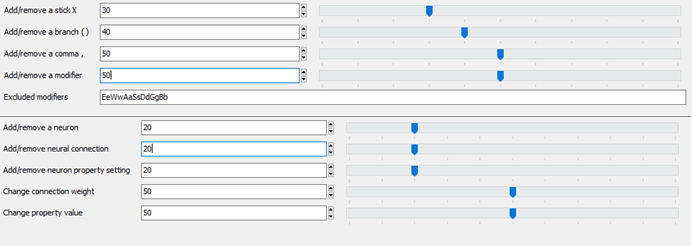
\includegraphics[scale=0.7]{f1params-starting}
    \label{fig:params}
    \caption{Default parameters of f1 encoding for the experiment.}
\end{figure}
\subsection{Modification 1}
Modifications:
\begin{itemize}
	\item No crossover;
	\item Selection - unchanged 40\%;
	\item Selection - mutated 60\%;
\end{itemize}
\begin{figure}[H]
	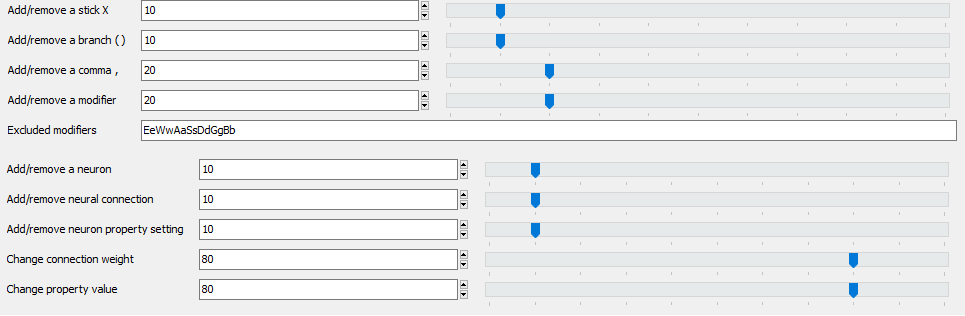
\includegraphics[scale=0.5]{f1params-mod }
	\label{fig:paramsmod1}
	\caption{Modified parameters of f1 encoding for the experiment (mod 1).}
\end{figure}
\subsection{Modification 2}
Modifications:
\begin{itemize}
	\item Gene pool - raised from 200 to 1000;
\end{itemize}
\section{Experiment}
Firstly, we tried creating an initial population with the below script, but when we investigated convergence of basic initial genotype compared to our code-generated, we found out that we worsened convergence, so we returned to using basic initial genotype.
\begin{minted}[fontsize=\scriptsize]{python}
  import random 
  def random_creature():
	 parts = ["R", "C", "L", "M", "c", "RR", "MM"]
	 num_parts = random.randint(3,10)
	 neurons_position = random.sample(range(num_parts),random.randint(0,num_parts))
	 neuron_count=0
	 split_stack = []
	 creature="("
	 for j in range(num_parts):
	  #chance to add split
	  if random.randint(0,100)<30:
	    creature+="("
	    split_stack.append("(")
 	  if random.randint(0,100)<60:
	    creature+=","*random.randint(1,2)
	  #add modificators to part
	  creature+= "".join(random.sample(parts, random.randint(1,3)))
	  #add part
	  creature+="X"*random.randint(1,3)
	  #adding neuron
	  neuron=""
	  valid_places = list(range((-neuron_count),len(neurons_position)-neuron_count))
	  if j in neurons_position and neuron_count!=len(valid_places):
	   neuron_count+=1
	   neuron +="["
	   #rotation muscle or bending
	   neuron += "".join(random.sample(["@", "|"], 1))
	   #add to body
	   for k in sorted(random.sample(valid_places, random.randint(1,len(valid_places)))):
	    neuron +=f"{k}:{random.randint(0,10000)/1000},"
	   neuron=neuron[:-1] #legacy code
	   neuron+="]"
	 creature+=neuron
	 #chance to close split
	 if len(split_stack)!=0 and random.randint(0,100) <20:
	  creature+="),"
	  split_stack = split_stack[:-1]
	 #adding splits
	 for _ in range(len(split_stack)+1):
	   creature+=")"
	 return creature
	
	
\end{minted}
By experimenting we got the following results:
\subsection{Default}
\begin{figure}[H]
	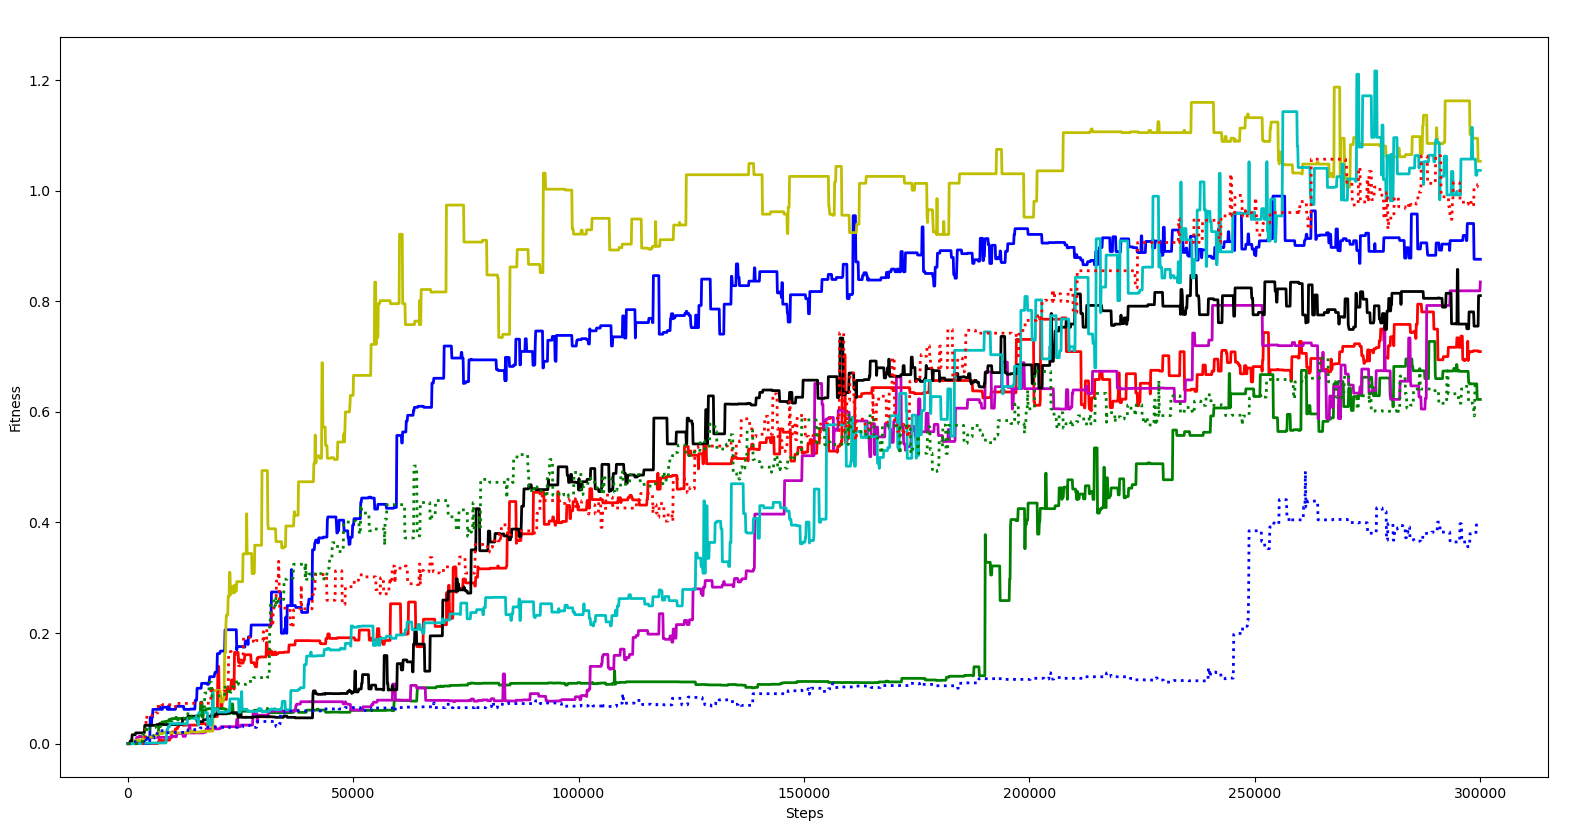
\includegraphics[scale=0.31]{def }
	\label{fig:def}
	\caption{Maxes plot of 10 runs for the default params.}
\end{figure}
\begin{figure}[H]
	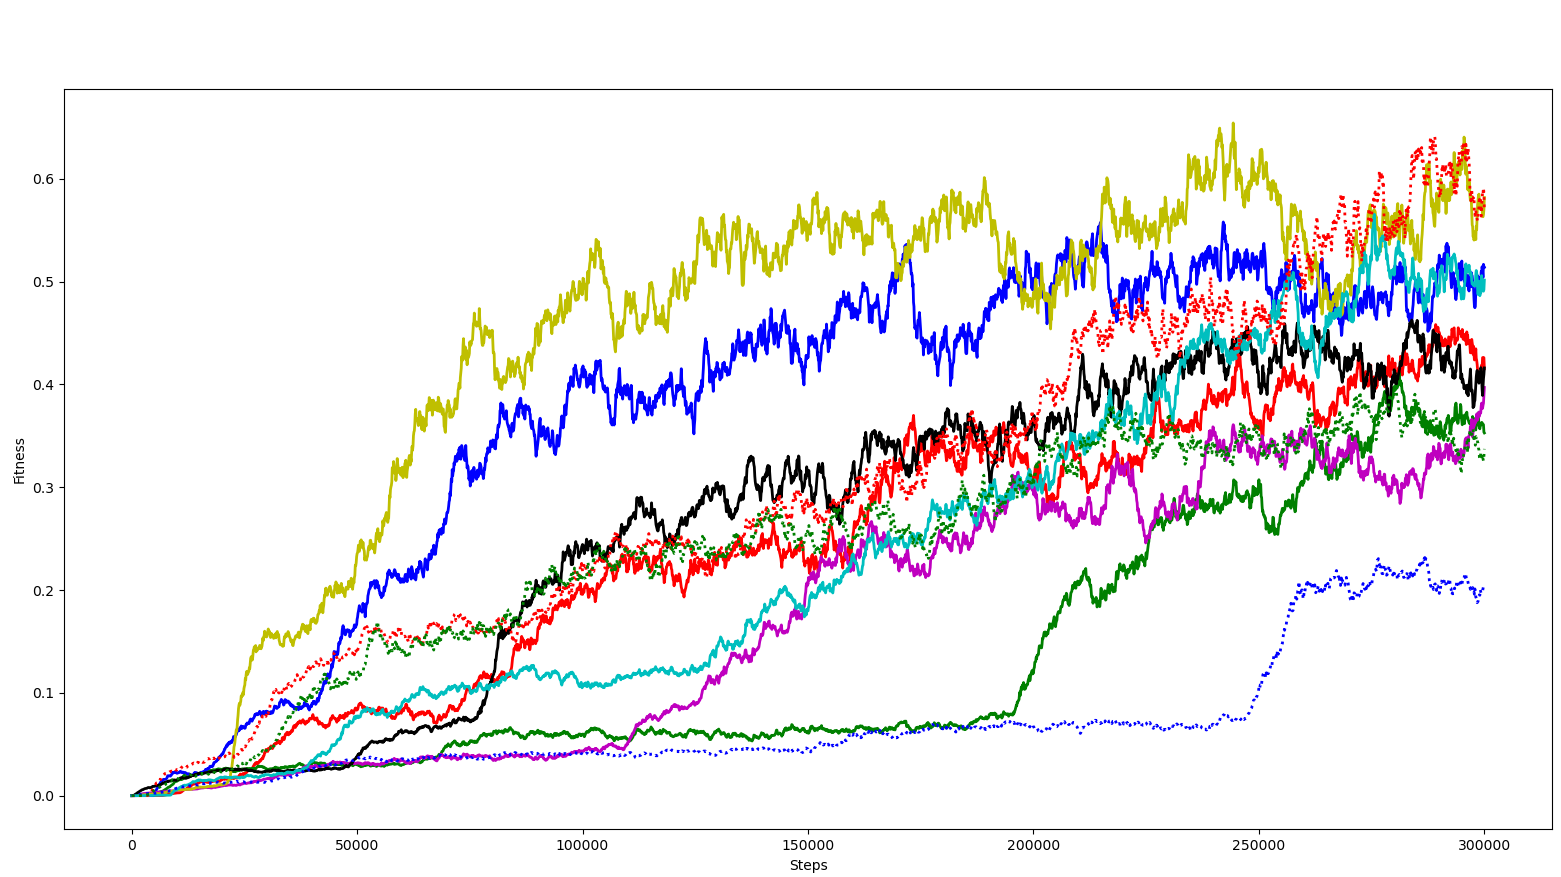
\includegraphics[scale=0.31]{avdef}
	\label{fig:defav}
	\caption{Averages plot of 10 runs for the default params.}
\end{figure}
\subsection{Modification 1}
\begin{figure}[H]
	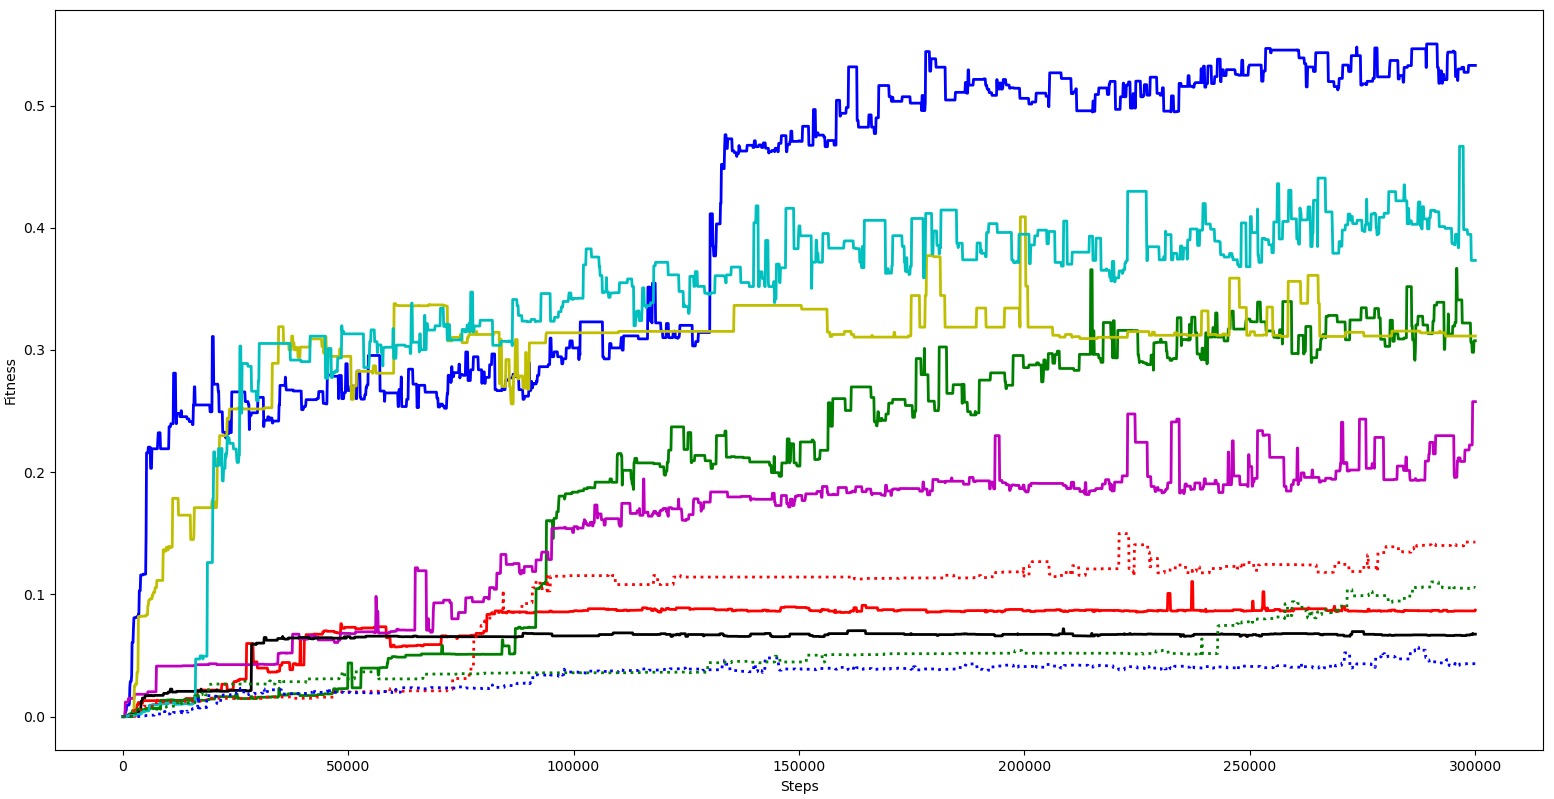
\includegraphics[scale=0.31]{mod1}
	\label{fig:m1}
	\caption{Maxes plot of 10 runs for modification 1.}
\end{figure}
\begin{figure}[H]
	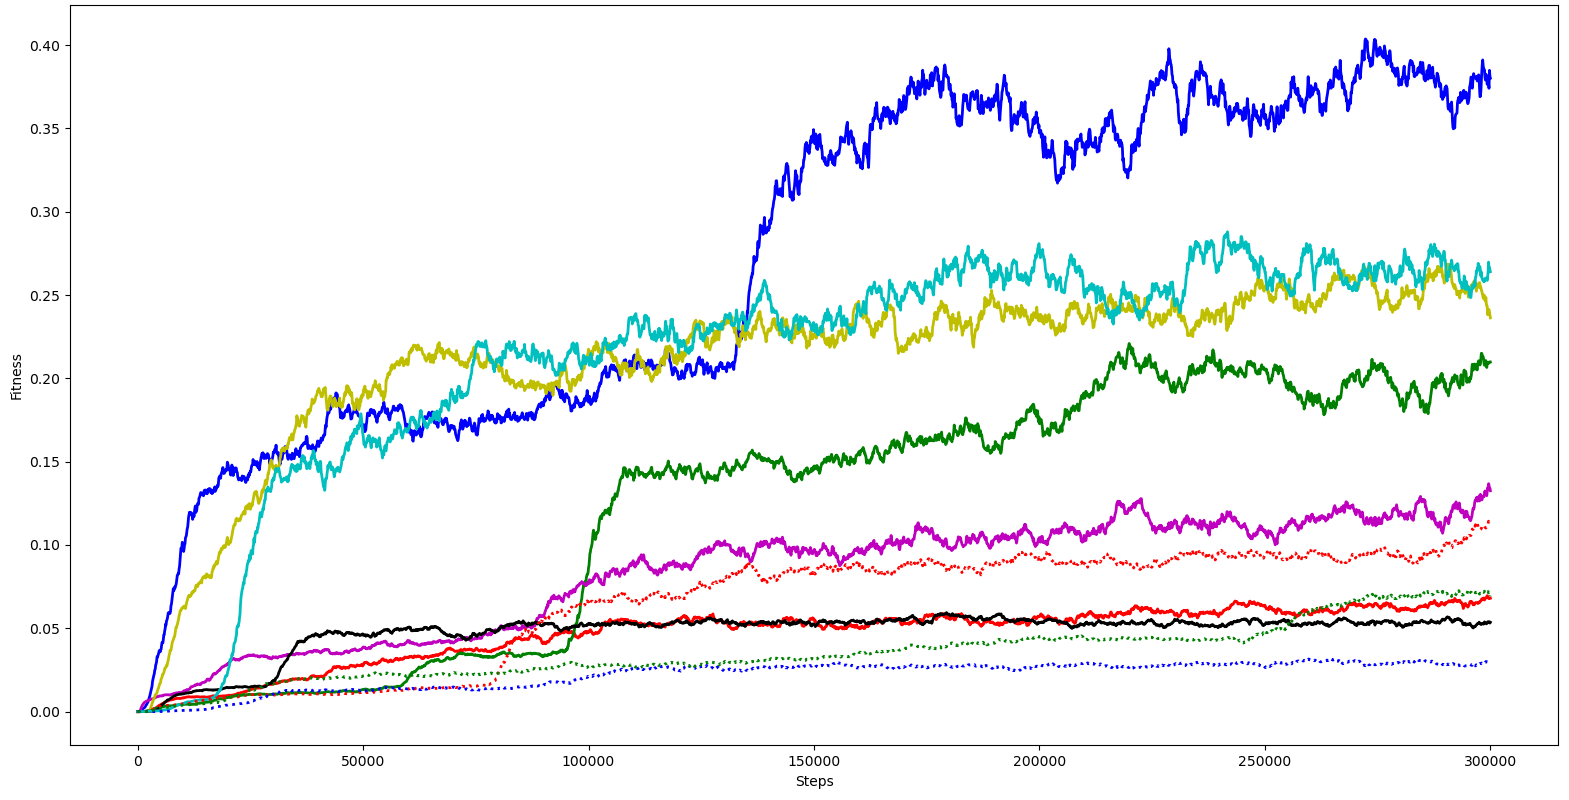
\includegraphics[scale=0.31]{avmod1}
	\label{fig:m1av}
	\caption{Averages plot of 10 runs for modification 1.}
\end{figure}
\subsection{Modification 2}
\begin{figure}[H]
	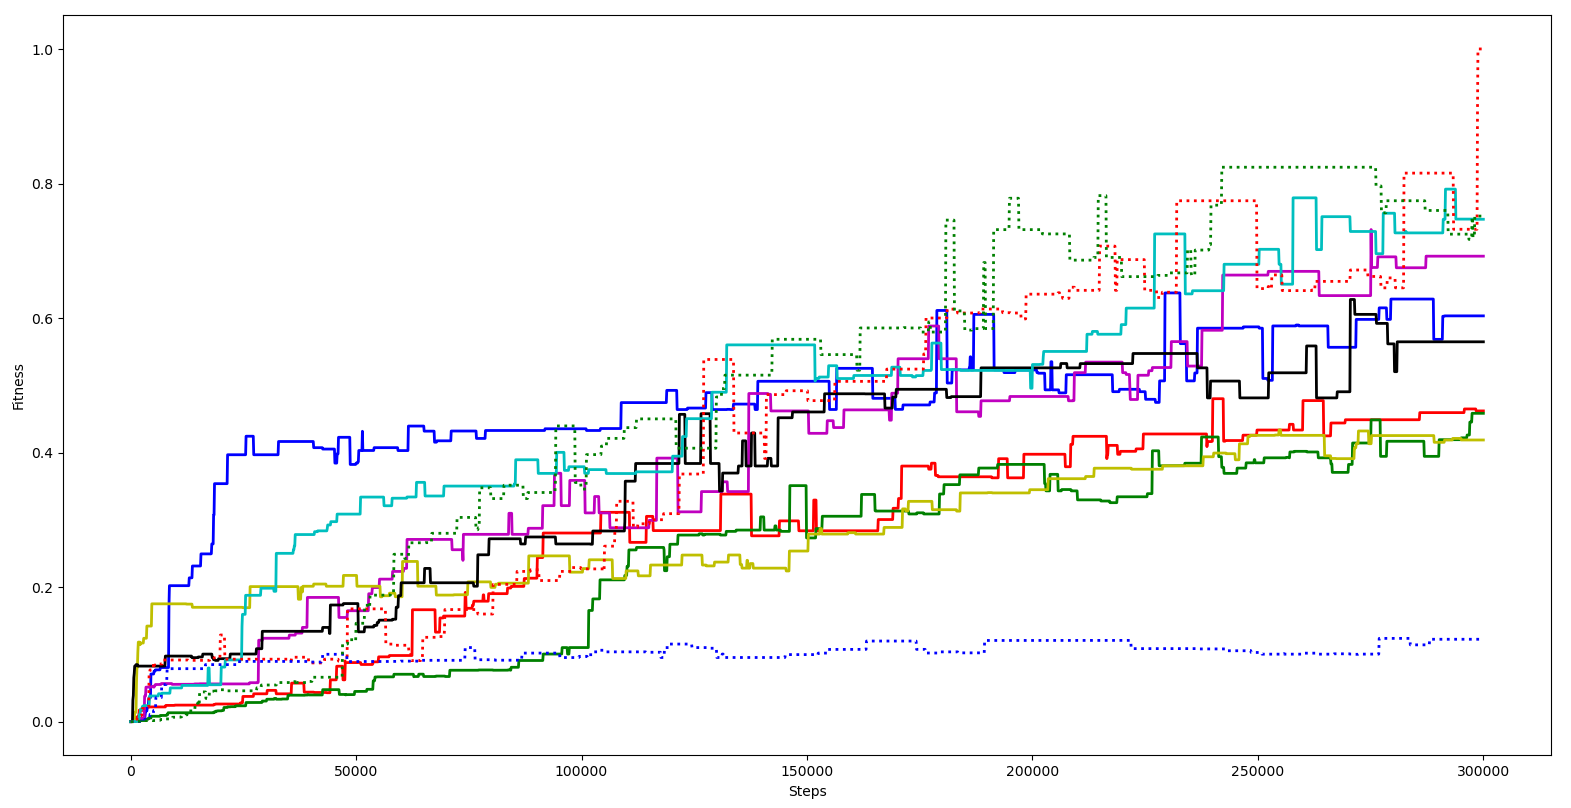
\includegraphics[scale=0.31]{mod2 }
	\label{fig:m2}
	\caption{Maxes plot of 10 runs for modification 2.}
\end{figure}
\begin{figure}[H]
	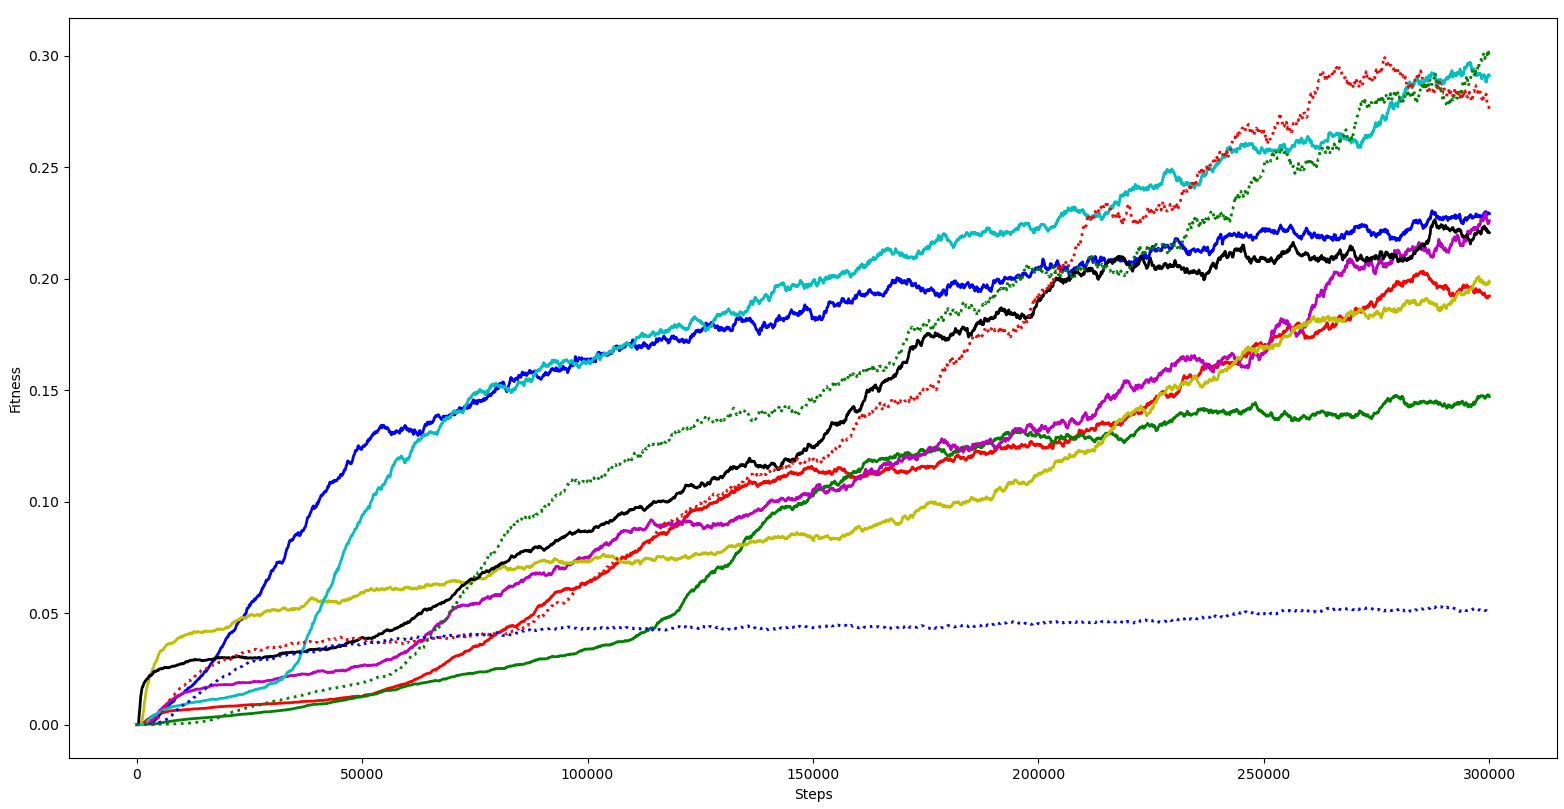
\includegraphics[scale=0.31]{avmod2 }
	\label{fig:m2av}
	\caption{Averages plot of 10 runs for modification 2.}
\end{figure}
\pagebreak
Violin plot for comparing fitnesses of different parameter combinations:
\begin{figure}[H]
	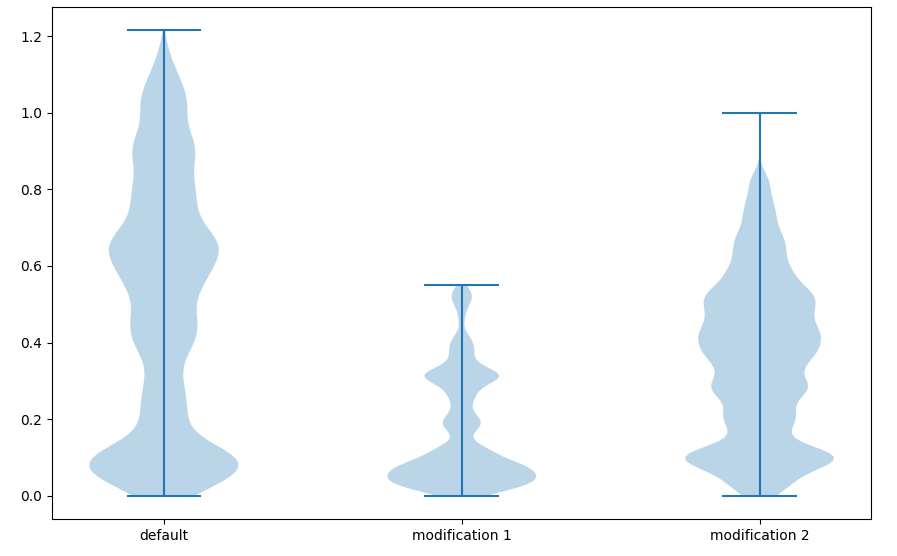
\includegraphics[scale=0.5]{michalskrzypek}
	\label{fig:michalskrzypek}
	\caption{Violin plot for the comparison of parameters}
\end{figure}
\section{Quantitive conclusions}
Based on the violin plot and fitness-in-time plots we can say that:
\begin{itemize}
	\item There was a significant breakthrough in fitness at least once during each run (as visible on figure 3). It can be caused by successful mutation i.e. adding working bending muscle.
	\item The evolutionary goal is not very hard so the oftentimes average fitness has steady, linear growth (as visible on figure 8).
	\item This is not a surprise that sometimes invalid genotypes occur or that the minimal fitness drops to near-zero values because not all mutations and crossovers are perfect. Bad ones can totally destroy working solutions and produce such outputs.
	\item There is room for improvement, the experiment can be run longer and produce much more interesting solutions. The chosen stopping criterion seems to be too strict.
	\item There are many short plateaus, places with no improvement, in each run but our default parameters seem to cope well with those local optima (as visible on figure 5). 
	\item Modification 1 sometimes gets stuck at local optima and cannot break through and performs much worse than default parameters (as visible on figure 5).
	\item Modification 2 is a simple gene pool increase but the fitness drops compared to the initial gene pool setting (as visible on figure 7).
\end{itemize} 
\section{Qualitative conclusions}
\textbf{What is the behavior of the best creatures?} \\
The best creatures try to use jump as a moving factor. They tend to jump at 20-30 degrees to travel as much distance as possible. \\
\\
\textbf{Do they have some special genotypes?} \\
The best creatures are minimalistic, avoiding unnecessary mass. Usually, they consist of 3-5 parts and 2-3 muscles forming a stick that can bend and rotate in 2/3 its length to break out of the ground. \\
\\
\textbf{Are the results in line with your expectations? If not, why?} \\
Yes, the results are not exactly in line with our expectations, especially since we thought that jumping at 45 degrees is optimal from a mathematical point of view. \\ \\
\textbf{Most representative creatures} (uploaded on YouTube, click on its name to open hyperlink):
\begin{itemize}
	\item \href{https://youtu.be/IhmRtiFgemY}{Framstick 1}
	\item \href{https://youtu.be/7Hn87hwG9KA}{Framstick 2}
	\item \href{https://youtu.be/XFscjOizwvY}{Framstick 3}
\end{itemize}
\listoffigures
\end{document}